
\documentclass[9pt,sigconf]{acmart}

\usepackage{color}
\usepackage{graphicx}
%\usepackage[justification=centering]{caption}
%\usepackage{subcaption}
%\usepackage{cite}


\usepackage{amssymb,amsmath}
%\renewcommand{\baselinestretch}{1.0}
%\setlength\floatsep{1pt plus 0.5pt minus 0.5pt}
%\setlength\textfloatsep{0pt plus 1pt minus 1pt}

\makeatletter
\def\hlinewd#1{%
\noalign{\ifnum0=`}\fi\hrule \@height #1 %
\futurelet\reserved@a\@xhline}
\makeatother
\usepackage{booktabs}
\usepackage{multirow}

\usepackage[binary-units=true]{siunitx}

%\usepackage[algoruled,noline,longend,linesnumbered]{algorithm2e}
%\setlength{\algomargin}{2.5em}
%\SetNlSkip{1.2em}
%\SetNlSty{textbf}{L}{}

\makeatletter
\def\hlinewd#1{%
  \noalign{\ifnum0=`}\fi\hrule \@height #1 %
\futurelet\reserved@a\@xhline}
\makeatother
\usepackage[tworuled,noline,linesnumbered]{algorithm2e}
\setlength{\algomargin}{2.0em}
\SetNlSkip{0.9em}
\SetNlSty{textbf}{L}{}
\SetAlFnt{\footnotesize}
\SetAlCapFnt{\footnotesize}
\SetAlCapNameFnt{\footnotesize} 


\usepackage{pgfplots}
\usepackage{pgfplotstable}
\usepackage{siunitx}
%\usepackage{tikz}


%\setlength\thinmuskip{0mu}
\setlength\medmuskip{3mu}
%\setlength\thickmuskip{0mu} 

%subparagraph not defined in IEEEtran but needed by titlesec
%\usepackage[compact]{titlesec}
%\titlespacing{\section}{0pt}{8pt}{2pt}
%\titlespacing{\subsection}{0pt}{6pt}{2pt}
%\titlespacing{\section}{0pt}{2pt}{1pt}
%\titlespacing{\subsection}{0pt}{2pt}{1pt}



%\setlength{\abovedisplayskip}{2pt plus 1pt minus 1pt}
%\setlength{\abovedisplayshortskip}{1pt plus 1pt minus 0.5pt}
%\setlength{\belowdisplayskip}{2pt plus 1pt minus 1pt}
%\setlength{\belowdisplayshortskip}{1pt plus 1pt minus 0.5pt}
\setlength\floatsep{10pt plus 0.5pt minus 0.5pt}
%\setlength\dblfloatsep{10pt plus 0.5pt minus 0.5pt}
%\setlength\intextsep{1pt plus 0.5pt minus 0.5pt}
\setlength\textfloatsep{3pt plus 1pt minus 1pt}
%\setlength\dbltextfloatsep{1.5pt plus 1pt minus 1pt}
\setlength\abovecaptionskip{3pt plus 0.5pt minus 0.5pt}
\setlength\belowcaptionskip{1pt plus 0.5pt minus 0.5pt}

%\makeatletter
%%change spaces around equations in amsmath
%\g@addto@macro\normalsize{%
  %\setlength\abovedisplayskip{2.8pt}
  %\setlength\belowdisplayskip{2.8pt}
  %\setlength\abovedisplayshortskip{-7.5pt}
  %\setlength\belowdisplayshortskip{0.8pt}
%}
%\makeatother

\setlength\evensidemargin{-2.3pc}
\setlength\oddsidemargin{-2.3pc}
\setlength\topmargin{-3.7pc}                % Nominal distance from top of
%%page to top of
%\textheight 666pt   %%original    % 9 1/4 column height
\setlength\textheight{689pt}
%\textwidth 42pc     %%original    % Width of text line.
\setlength\textwidth{43.8pc}         % Width of text line.
%\setlength\topmargin{-5.5pc}
%\setlength\columnsep{1pc}         %    Space between columns
\setlength\columnsep{1pc}         %    Space between columns

%
%%\makeatletter % access to internal commands
%%\renewcommand{\@seccntformat}[1]{\csname the#1\endcsname\ }
%%%\makeatother

%\setcounter{page}{1}
%\pagestyle{fancy}
%\renewcommand{\headrulewidth}{0pt}
%\fancyhf{}
%\rfoot{\small \thepage/\pageref{LastPage}}
%\rhead{\small \thepage}
%\setcopyright{acmcopyright}

%\setcopyright{rightsretained}
\settopmatter{printacmref=false} % Removes citation information below abstract
%\renewcommand\footnotetextcopyrightpermission[1]{} % removes footnote with conference information in first column
%\pagestyle{plain} % removes running headers


\copyrightyear{2018}
\acmYear{2018}
\setcopyright{acmcopyright}
\acmConference[DAC '18]{DAC '18: The 55th Annual Design Automation Conference 2018}{June 24--29, 2018}{San Francisco, CA, USA}
\acmBooktitle{DAC '18: DAC '18: The 55th Annual Design Automation Conference 2018, June 24--29, 2018, San Francisco, CA, USA}
\acmPrice{15.00}
\acmDOI{10.1145/3195970.3196025}
\acmISBN{978-1-4503-5700-5/18/06}

\begin{document}

%\frontmatter
%\pagestyle{headings}
%\pagestyle{plain}


\graphicspath{{Fig/}}
\def\figname{Figure}
\def\algname{Algorithm}
%\def\algname{Procedure}
%\newcommand{\figurefontsize}{\fontsize{7.0pt}{1}\selectfont}
\newcommand{\figurefontsize}{\small}

\pagestyle{empty}

15 gid=3000000
15 uid=3603518
27 mtime=1539603730.121268
27 ctime=1539603730.122269
27 atime=1539603730.144268


\newcommand{\papertitle}{Design-for-Testability for Continuous-Flow Microfluidic Biochips}


\title{\papertitle}
%\author{
%  \vskip 10pt
 %Chunfeng Liu$^1$, Bing Li$^1$, Bhargab B. Bhattacharya$^2$, Tsung-Yi
%Ho$^{34}$, Ulf Schlichtmann$^1$\\
%$^1$Institute for Electronic Design Automation, Technical University of Munich (TUM), Munich, Germany\hfill\\
%$^2$Indian Statistical Institute, Kolkata, India\hspace{18pt}
%$^3$National Tsing Hua University, Hsinchu, Taiwan \hfill\\
%$^4$Institute for Advanced Study, Technical University of Munich (TUM), Garching, Germany\hfill
%}
%\author{}
%\institute{}
%\vskip 50em

\author{
Chunfeng Liu$^{1,4}$, Bing Li$^1$, 
Tsung-Yi Ho$^{2,4}$, 
Krishnendu Chakrabarty$^{3,4}$, 
Ulf Schlichtmann$^1$\\
\normalsize 
$^1$Chair of Electronic Design Automation, Technical University of
Munich, Germany\hskip 10pt $^2$National Tsing Hua University, Hsinchu, Taiwan \\
$^3$Department of ECE, Duke University, Durham, NC, USA \hskip 10pt 
$^4$Institute for Advanced Study, Technical University of Munich, 
Germany\\
\{chunfeng.liu, b.li, ulf.schlichtmann\}@tum.de, tyho@cs.nthu.edu.tw, krish@ee.duke.edu
}



\maketitle



15 gid=3000000
15 uid=3603518
27 mtime=1539604186.701956
26 ctime=1539604186.70196
27 atime=1539604186.703959


\section{Fault Model and Problem Formulation}\label{sec:formulation}

During manufacturing of flow-based biochips, various defects may occur. For
example,  the flow channel under a valve may be broken
and does not allow any fluid to pass, leading to a fault equivalent to the
case that the valve cannot be opened. In addition,  leakage may appear between
neighboring flow channels, so that fluids in them may be directed to incorrect
devices or mixed unexpectedly. Furthermore, if the control channel to a valve
becomes broken, air pressure  may not reach the valve. Consequently, this valve
cannot be closed and thus causes a constant leakage.  Furthermore, a leakage may
also appear between two control channels, so that  the valves they drive are
always opened and closed together. 
%another fault scenario leading to malfunction of the chip potentially. 
These cases of manufacturing defects are illustrated 
in \figname~\ref{fig:defects} from \cite{HuYHC14}.


%The defects in a manufactured flow-based biochip have been analyzed in detail
%and the corresponding fault models have been defined in \cite{HuYHC14}.

%Defects in manufactured biochips may cause malfunction in executing bioassays.
According to how the defects affect the behavior of a valve or a channel,
typical faults 
%at component level 
can be defined as follows:

\begin{itemize}

\item \textit{Broken flow channel}: Fluid cannot pass through a channel. This is
equivalent to the fault that the valve at the entrance of the channel cannot be
opened.  

\item \textit{Leaking flow channel}: Fluid in a channel leaks to its
  neighboring channel. In FPVAs, this fault is similar to the case 
  that a valve separating two cells cannot be closed. 

  %If a valve does not exist between the two channels with
  %leakage, such as in traditional biochips,  a virtual valve can be assumed
  %%between them and its state should be always closed. The leakage defect can
  %thus be covered if a test pattern identifies that this virtual valve needs to
  %be opened to realize the observed results. 

\item \textit{Broken control channel}: Valve cannot be closed.

\item \textit{Leaking control channel}: Two valves open or close simultaneously
  due to the shared air pressure in the control channels.

\end{itemize}
Since the faults that valves are stuck at the always-closed or always-open
states are similar to the stuck-at-0 faults and stuck-at-1 faults in digital
circuits, these faults are henceforth called \textit{stuck-at-0 faults}
and \textit{stuck-at-1 faults} for convenience.


\begin{figure}[t]
{\figurefontsize
\centering
\input{Fig/defects.pdf_tex}
\caption{Defects in flow-based biochips \cite{HuYHC14}. (a)
Broken flow channel. (b) Leaking flow channel. (c) Broken control channel. (d)
Leaking control channel.}
\label{fig:defects}
}
\end{figure}

With these fault models, test of traditional flow-based biochips has been
examined in \cite{HuYHC14}. The concept of this method can be explained
using the example illustrated in \figname~\ref{fig:classic_test}(a) from
\cite{HuYHC14}. In this test concept, a pressure source is connected to the
input port of the chip to create air pressure along the channels in the flow
layer. Pressure sensors are attached to the output ports of the chip to detect air
pressure. By switching the valves open or closed according to test patterns,
the air pressure read by the pressure sensors 
at the output ports can be used to determine whether
there is a fault in the chip. In this test process, an air pressure is applied
to the flow channels to detect faults, so that the chip is not
contaminated after test. This air pressure for the purpose of test 
is completely unrelated to the pressure applied in the control channels to 
switch valves when the chip executes bioassays.

In \figname~\ref{fig:classic_test}(a), an air pressure can only be detected at
an output port if there is a path from the pressure source to the output port. For example,
if only the valves $a, g, h, i, k$ are open,  a pressure can be detected
at $o_2$. However, during this test if a valve on this path cannot be opened due to
defects, no pressure can be detected at $o_2$, indicating the
existence of a stuck-at-0 fault. On the other hand, if a valve on this path is also
closed intentionally during the test, all paths from the source to the output
ports should be blocked,
so that no air pressure should be detected at any output port. If, on the
contrary, the test results show that a pressure can still be observed by a
sensor, a stuck-at-1 fault should exist in the chip to allow a path from the
source to an output port to be formed. In this test process,   
the states of the valves during a pressure actuation-measurement cycle is
called a \textit{test pattern}. It is the task of test generation to generate
as few test patterns as possible to detect the faults in a chip efficiently.

To generate test patterns, the method in \cite{HuYHC14} converts the
biochip under test into a circuit as shown in
\figname~\ref{fig:classic_test}(b), where the inputs of the circuit
represent valves and the outputs of the circuit represent the output ports
of the chip. In this circuit representation, valves along the same
channel segment are inputs of AND gates, e.g., $b, c, d, e, f$ and $g,
h$. If two channels converge at a point, 
%e.g., the two channels through $f$ and $h$, 
%e.g., the converging point between the valves $f, h, i$, 
an OR gate is created in the circuit representation, since a pressure through
any of these channels can reach the converging point. Consequently, 
the circuit represents the relation between valves and the paths from the source to
the output ports in the chip.
%defines the relation between valves in activating pressure at the output ports. 
%Therefore, 
To generate test patterns for the biochip, it is
equivalent to generate test patterns for the circuit representation, which can
be achieved by a standard ATPG tool as shown in \cite{HuYHC14}.

%In addition to valve faults,  the ATPG-based method can also efficiently deal
%with channel leakage faults. A flow channel leakage fault leads to two channel
%segments being filled with fluid at the same time if one of them is filled. 
%This is equivalent to the case that if a node in the test circuit is `1',
%another node is also `1', an OR-bridge fault in the circuit representation.  If
%there is a leakage in the control channel, two valves close simultaneously if
%one of them is closed. This is an AND-bridge fault in the circuit.  By using
%the equivalent circuit test structure, both bridge faults can be tested with
%ATPG vectors efficiently.

The ATPG-based method has the advantage that the biochip under test needs only
to be converted into a circuit representation. The real test generation is
performed using test generation methods for integrated circuits.
However, it is challenging to apply this method directly to test FPVAs
shown in \figname~\ref{fig:archi}(a).  
In converting a biochip into a circuit representation, the structure of the chip
should be known.
%the relation between valves should be known. This relation is defined by 
%path information from the pressure source to the output ports. 
On an FPVA, the shapes and locations of devices and transportation
channels are dynamically determined according to the operations to be executed.
%there is no such a path structure, because all devices are created dynamically
%according to the operations to be executed. 
If the ATPG-based method is still applied, it then needs to cover 
a huge number of dynamic chip architectures, which is 
a challenging task in view of the flexibility of FPVAs.

\begin{figure}[t]
{\figurefontsize
\centering
\input{Fig/ref_test_biochip.pdf_tex}
\caption{Test of traditional flow-based biochips \cite{HuYHC14}. (a)
Schematic of the chip under test. (b) Circuit representation of the test 
model for test pattern generation.}
\label{fig:classic_test}
}
\end{figure}

In this paper, we propose a new test framework for detecting faults in an FPVA
%a manufactured chip reliably 
with only a small set of test patterns. This problem can be formulated as follows:
\begin{itemize}

  \item{Input:} An FPVA architecture; the locations of long channels (no valve
    built, conceptually always open) and obstacles (conceptually always
    closed); the locations of the air pressure source and the pressure sensors.

\item{Output:} A set of test patterns, each of which defines the
open/closed states of all valves when test pressure is applied
at the source and checked at the output ports by the pressure sensors.

\item{Objective:} The number of test patterns should be 
  as small as possible to reduce test cost; faults should be detected reliably by
  covering all valves.
  %the number of undetected faults should be as small as possible.

\end{itemize}


%\section{Design-for-Testibility with }
\section{Constructing Design-for-Testability Biochip Architecture}\label{sec:dft_arch}

In this section, we explain the strategy and the implementation to generate an 
augmented biochip architecture and the corresponding test vectors.
%and the schedule of the application on the new architecture.

As observed in \figname~\ref{fig:multiPortSingPort}, a biochip with multiple
ports can obtain single-source single-meter testability by adding additional
DFT channels and valves.  In the proposed method, the locations of these
channels and valves are determined by mapping the input chip architecture to a
virtual connection grid, as shown in \figname~\ref{fig:fitintogrid}. In this
mapping, devices are assigned to nodes and channels to edges in the
grid, while keeping the original topology of the chip unchanged.  After this
mapping, the nodes and edges that have not been occupied in the connection
grid represent the possibilities where additional channels and valves can be
built. 
In the mapping in \figname~\ref{fig:fitintogrid}, valves need not to be mapped
to the nodes explicitly,
%included, 
because they are needed only at the inputs/outputs of devices and the crossing
points between channels and they are tested together with valves.
%automatically when channels are tested.

%. The testing vectors enable flow paths to
%test stuck-at-0 defects. If a path covers several segments of the
%transporation channels, the valve on them are tested automatically. For
%example, alougth the vavles on the test path P1 do not appear in the
%connection grid, a stuck-at-0 defect on them can still be detected because no
%pressue can be measured at the pressure meter.  Therefore, the channels need
%only to be inserted back after DFT channels are created.  

The 
%single-source single-meter 
testability of stuck-at-0 defects of a biochip requires that for each valve or
channel, there is a path from the single pressure source to the single
pressure meter.  In the proposed method, we use this requirement to identify
the locations of new channels and valves. Afterwards, test cuts are
generated from the augmented architecture to test stuck-at-1 defects.

For a given biochip architecture, there might be multiple possibilities to add
channels and valves to implement the single-source single meter testability.
In the following, a feasible solution of this testability problem is called a
\textit{DFT configuration}. In the proposed method, we identify the DFT
configurations using Integer Linear Programming (ILP) programming.

Assume there is a path $p_r$ between nodes $n_{s}$ and $n_{t}$, which
represent the locations of the external ports 
%of the given biochip mapped onto 
on the connection grid. We use a 0-1 variable $e_{j,r}$ to represent whether
the edge $e_j$ in the connection grid is on the path $p_r$, and the 0-1
variable $n_{i,r}$ to represent whether the node $n_i$ is on the path $p_r$.
For nodes $n_{s,r}$ and $n_{t,r}$, only one of the four edges incident to it 
%to each of them 
can be covered by the path $p_r$.  
%a node $n_i$ on a test path between 
At each other node $n_i$ on the path, exactly two edges incident to it are
covered.  Accordingly, we can construct the path with the following
constraints,
\begin{align}\label{eq:path_construct} 
% \sum_{e_j\in E_s}e_{j,r}=\sum_{e_j\in E_t}e_{j,r}=1,\quad 
 \sum_{e_j\in E_i}e_{j,r} = 2n_{i,r} ,\quad \forall n_i\in N, n_i \ne n_{s}, n_{t}\\ 
  \sum_{e_j\in E_i}e_{j,r} = 1, \quad  \forall n_i = n_{s}, n_{t}
\end{align}
where 
%$E_s$, $E_t$ and 
$E_i$ is the set of edges incident to the node 
$n_i$ and $N$ is the set
of all the nodes in the connection grid.

\begin{figure}
\figurefontsize
\centering
%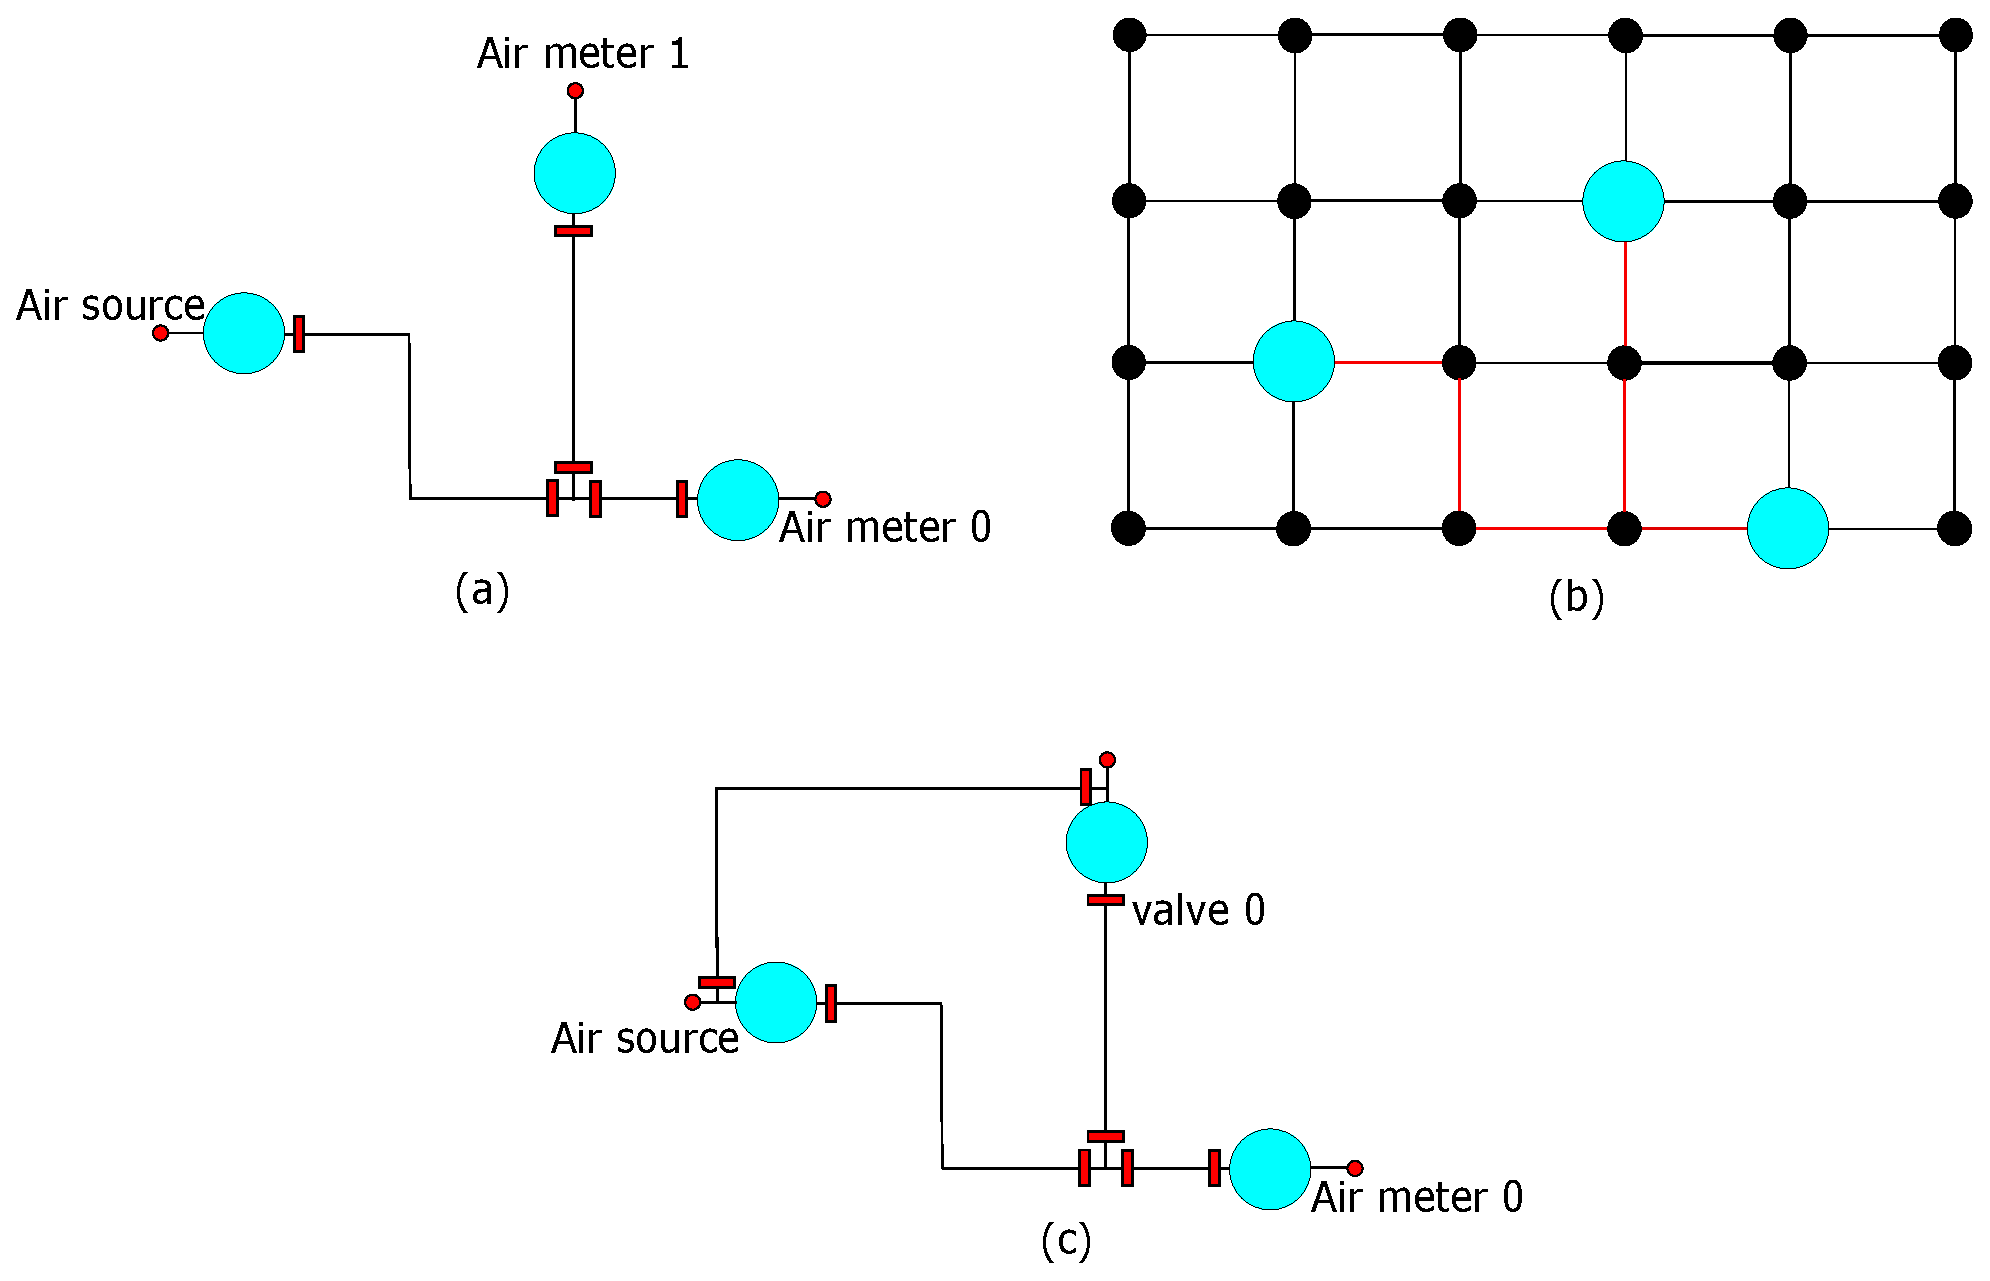
\includegraphics[width=3.50in,height=2.2in]{Fig/fitintogrid2.eps}
\input{Fig/grid.pdf_tex}
\caption{Mapping a biochip onto a virtual connection grid.}
%(a) Origin biochip. (b) Connection grid after mapping. Thick edges 
%represent the edges occupied by the original channels.}
%(c) Design-for-test architecture}
\label{fig:fitintogrid}
\end{figure}


Since the channel segments occupied by the original chip must appear in the new
architecture, the constraints for these edges can be written as
\begin{equation}\label{eq:edge_cover}
\sum_{p_r\in P} e_{j,r}\ge 1,\quad \forall e_j\in E_{o} 
\end{equation}
where $P$ is the set of all test paths; $E_{o}$ is the set 
of edges occupied by the original channels in the connection grid.

When generating the DFT architecture of the chip, we minimize the number of
added channels.
We use a 0-1 variable $s_j$ to represent whether the edge $e_j$ in the connection
grid should be kept in the final chip. If any test path covers $e_j$, $s_j$
must be 1, so that the relation between $s_j$ and $e_j$ can be established as
\begin{equation}\label {eq:edge_used} 
  s_j\ge e_{j,r}, \quad \forall p_r\in P, \quad \forall e_j \in E \backslash E_{o}
\end{equation} 
where $P$ is the set of all test paths and $E \backslash E_{o}$ 
represents the set of edges in the connection grid that are not covered by the original
chip.

Finally, the architecture of the DFT chip can be determined by solving the
following optimization problem
\begin{align} \label{eq:DFT_opt_1}
\text{minimize} & \quad \sum_{e_j\in E\backslash E_{o}}s_j\\
\text{subject to} & \quad
\text{(\ref{eq:path_construct})--(\ref{eq:edge_used})}.\label{eq:DFT_opt_2}
\end{align}

In this optimization, the number of potential test paths $|P|$ should be
determined in advance. This number should be large enough to cover all the
channels in the augmented architecture. In the implementation, we started by
setting this number to 2, and increased it by 1 in the next iteration when the current number
produces no valid result. Another issue is that the formulation above assumes
that starting and ending nodes of paths are given. Although any two ports in
the chip are feasible test ports in the final DFT architecture, we used the
two ports between which the distance is the largest to generate long instead
of short test paths, so that more channels and devices in the original chip
can be covered by an individual path potentially. The last issue of the
formulation above is that loops may be generated on the paths. These loops
need to be excluded to avoid false coverage of the original channels and
devices. In the proposed method, we used the technique in
\cite{LLHS17} to exclude these loops.

%\subsection{Test Vectors and Application Scheduling}

In generating DFT valves and channels above, the test paths to detect
stuck-at-0 defects have been created simultaneously. The stuck-at-1 defects
are detected by test cuts applied to the chip. A cut is composed of a
set of valves which separate the port connected to the pressure source and the
port connected to the pressure meter during test.  After test paths are
created for single-source single-meter test, test cuts can always be created
successfully because in the worst case test paths can be blocked individually
to form cuts. The problem to find the minimum set of test cuts for a given
biochip is a complementary problem of the test path generation
%in Section~\ref{sec:dft_arch} 
so that the details are omitted due the page limit.  


\input{valve_sharing}
15 gid=3000000
15 uid=3603518
27 mtime=1539614027.556887
27 ctime=1539614027.557883
27 atime=1539614027.558899

15 gid=3000000
15 uid=3603518
27 mtime=1539178688.491291
27 ctime=1539178688.491292
27 atime=1539178688.494292

\section*{Acknowledgment}

The work of B. Li and U. Schlichtmann was supported by Deutsche
Forschungsgemeinschaft (DFG) through TUM International Graduate School of
Science and Engineering (IGSSE).
%The work of B. B. Bhattacharya was supported, in part, by the
%special research grant funded by PPEC, Indian Statistical Institute,
%Kolkata.
The work of C. Liu was supported fully, and the work of 
K. Chakrabarty and T.-Y. Ho was supported in part, by the Technical University
of Munich -- Institute for Advanced Study, funded by the German
Excellence Initiative and the European Union Seventh Framework Programme under
grant agreement n$^\circ$ 291763.
%The work of T.-Y. Ho was also supported in part by the Ministry of Science and Technology of
%Taiwan, under Grant MOST 105-2221-E-007-118-MY3.





%\let\oldthebibliography=\thebibliography
%\let\endoldthebibliography=\endthebibliography
%\renewenvironment{thebibliography}[1]{%
%\begin{oldthebibliography}{#1}%
%%\setlength{\itemsep}{0ex}%
%%\def\baselinestretch{1}
%\fontsize{8.0pt}{1}\selectfont
%\vskip 1pt
%\scriptsize
%\small
%\footnotesize
%\reffontsize
%\newlength{\mylength}
%\setlength{\mylength}{7.5pt}
%\setlength{\baselineskip}{\baselinestretch\mylength}
%\setlength{\baselineskip}{30pt}
%}%
%{%
%\end{oldthebibliography}%
%}


%%\renewcommand{\baselinestretch}{2} 
\let\oldthebibliography=\thebibliography
\let\endoldthebibliography=\endthebibliography
\renewenvironment{thebibliography}[1]{%
\begin{oldthebibliography}{#1}%
\vspace{3pt}
%%\setlength{\parskip}{0ex}%
%\setlength{\itemsep}{0ex}%
%%%%%%bil
\fontsize{7.0pt}{1}\selectfont
%%\vskip 1pt
%\scriptsize
%%\small
%\reffontsize
}%
{%
\end{oldthebibliography}%
}

%\bibliographystyle{abbrv}
%\bibliographystyle{unsrt}


\bibliographystyle{IEEEtran}
%\bibliographystyle{ACM-Reference-Format}
\bibliography{IEEEabrv,CONFabrv,bibfile}

\end{document}


